\section{Legal and Ethical Issues}
The research project was conducted with ethical considerations where safety and well being of researcher and participants was considered seriously. The Ethics Board has approved the research project for developing a convolutional neural network to detect pigmented skin lesions with ethics id P101878. Due to the current pandemic spread of coronavirus, it was not safe to visit hospitals. As a result, the data collection was performed through the online exchange of forms. The research project involves detecting skin cancer from pigmented skin lesions for which publicly available dataset was used with any personal identity of any patient information which might have ethical considerations to collect data from medical professionals. 
The participants of the study were completely aware of the purpose of the study. The data collection process of secondary research was compliant with GDPR privacy laws in the united kingdom. The documents containing information collected from participants were stored in the password-protected the document and will be destroyed after the research submission. The participants of the research project were informed that they could withdraw their data at any time without any reason or mental pressure. The consent formed was attached to the questionnaire, which required participants to give permissions to collect the data and related concerns.

\section{Research Challenges}
There were various challenges while conducting the research to develop and compare 
the automated system for classification of pigmented skin lesions. The risk of no 
prior knowledge about the convolutional neural network was present in the initial phase 
which required the personal research on foundations of artifical neural network and 
learning to operate the keras deep learning library. The research involved performing 
the image processing and normalisation tasks which requires the superior hardware 
the 8 gigabytes of the RAM (random access memory) was not suffient to normalise the 
original images from the dataset and train the VGG16 network. As, a result the images were resized to 224 * 224 pixels to 
reduce the consumption of the primary memory. Furthermore, the VGG16 model was 
trained on the google colab platform which provides free computation power to 
train the artifical neural networks. However, the colab platform requires the user  to 
interact with the web interface to avoid timeout error. The secondary research for the 
project involves comparing the data collected from the medical professionals with 
automated system. However, due to the pandemic coronavirus it was not safe to 
collect the data from medical hosiptals which resulted in fewer resulted in fewer 
responses from the medical professionals.

\pagebreak

\section{Project Managment}

\subsection{Software Development Lifecycle}

\begin{figure}[!htp]
    \centering
    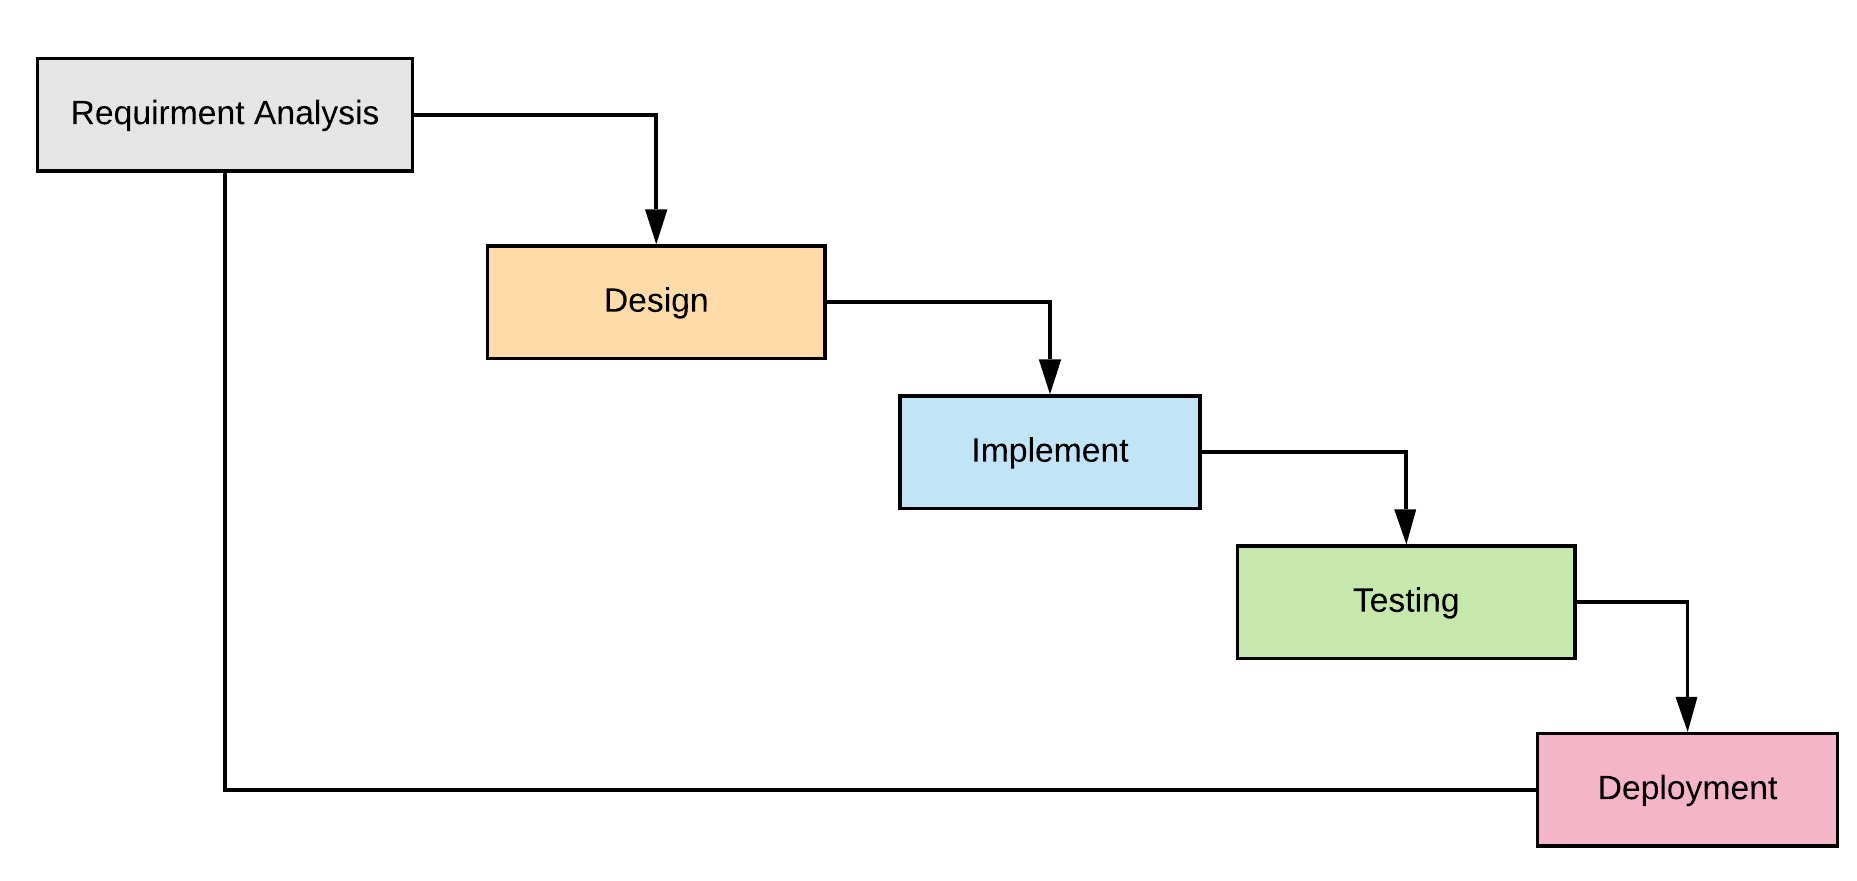
\includegraphics[width=.8\textwidth]{Images/waterfall}
    \caption{Waterfall Model}
    \label{fig:waterfall}
\end{figure}


The waterfall software development lifecycle was used during developing the project. The waterfall
model also known as linear-sequential life cycle model focuses on completing each phase of
development before switching to the next stage of development Cite{1}. The waterfall model was
accurate for this project as the scope of the project is small and was developed individually. Output
from each phase of development lifecycle acts as the input to the next phase. The figure above
\ref{fig:waterfall} shows the various phases of the waterfall development lifecycle. In initial phase of the
development the requirements and targeted audience were analysed as mentioned in the
introduction section of the project. The second phase involved developing conceptual models using
UML(Unified Modelling Language) to design the system using component diagram which captures
the structural and sequence diagram to capture the behavioural design of the system. The next
phase of waterfall model was implementation of the intelligent system to detect pigmented skin
lesions. The implementation phase of the lifecycle involved developing convolutional network and
performing various experiments to get optimal performance. Furthermore, The next phase of
development was to test the effectiveness of the overall system for which the prediction results
gathered from medical professionals in the form of questionnaires were compared with the
automated system and results were analysed with confusion matrix. The last phase was to deploy
the model to the web-based system which was done by converting the keras model to json file and
using tensorflowjs. At last, the maintenance phase of lifecycle cannot be applied to short term
project.

\pagebreak
\subsection{Work Managment System}
\begin{figure}[!htp]
    \centering
    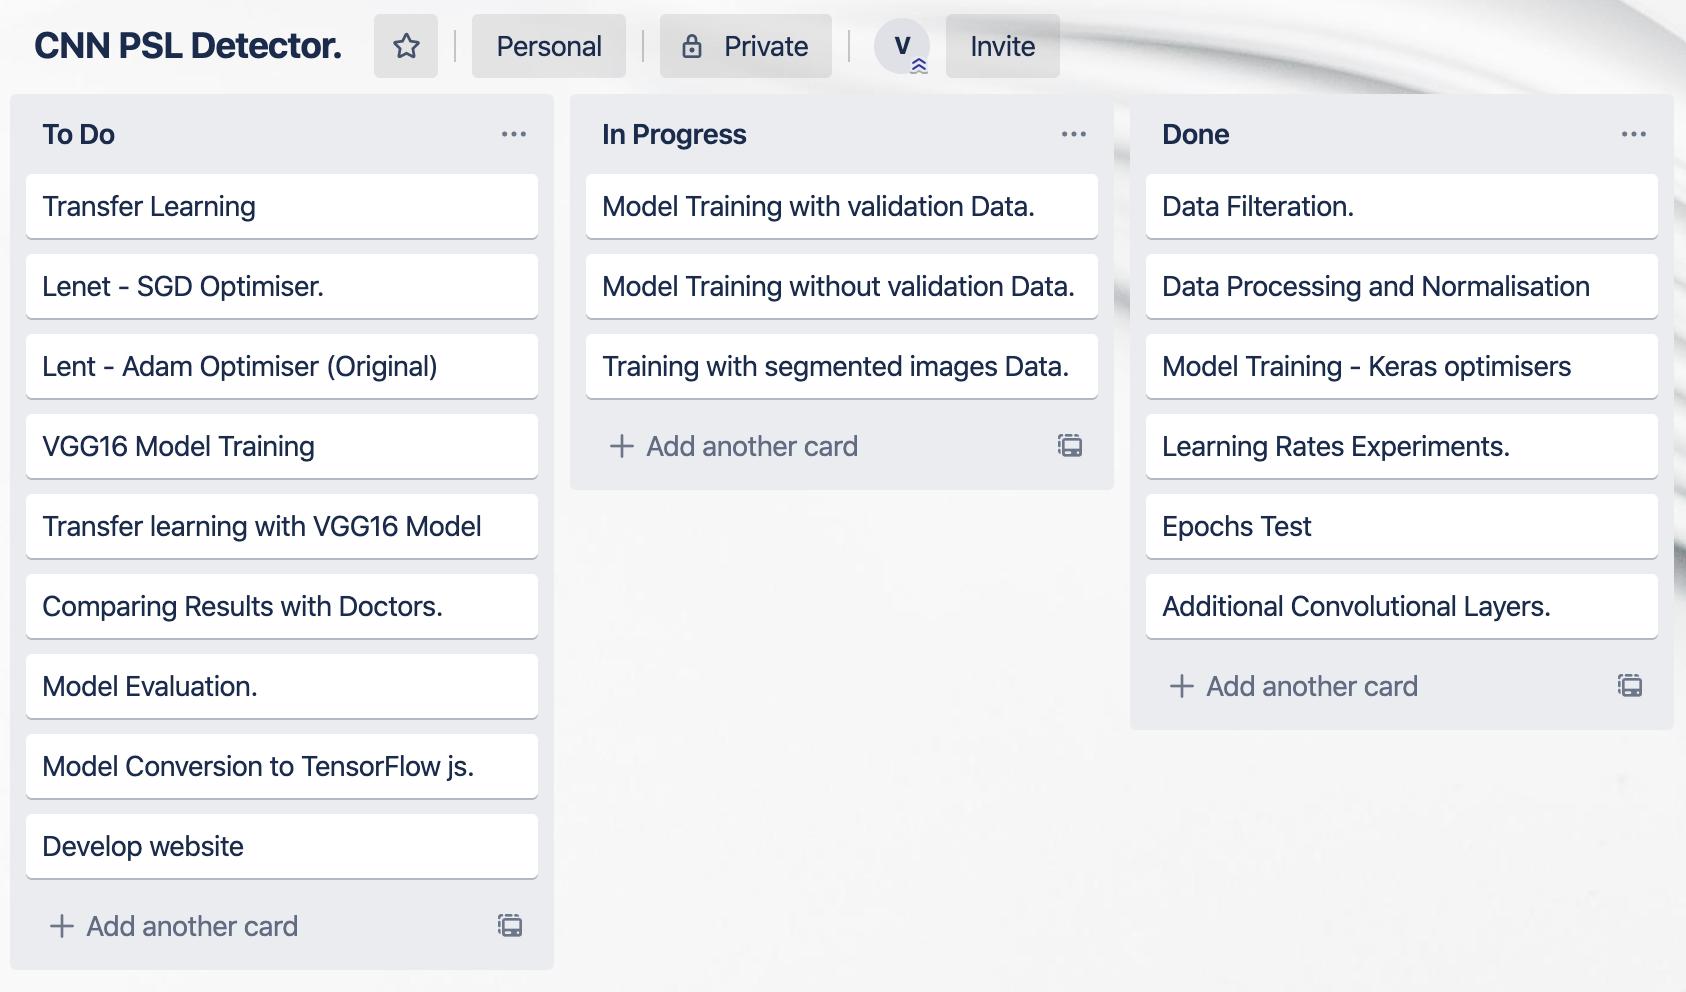
\includegraphics[width=15cm]{Images/Kanban Bords.png}
    \caption{Kanban Board}
\end{figure}
\pagebreak
\subsection{Response to Supervisor Feedback}
\pagebreak


